\documentclass[12pt]{article}
\usepackage[utf8]{inputenc}
\usepackage{graphicx}
\graphicspath{ {./plot/} } % Uncomment
\usepackage[
top=2cm,
bottom=2cm,
left=2cm,
right=2cm,
headheight=17pt, % as per the warning by fancyhdr
includehead,includefoot,
heightrounded, % to avoid spurious underfull messages
]{geometry} 
\geometry{a4paper}
\usepackage{fancyhdr}
\usepackage{float}

% Lecture Name, exercise number, group number/members
\newcommand{\lecture}{GPU Computing}
\newcommand{\exercise}{Exercise 7}
\newcommand{\groupnumber}{gpucomp03}
\newcommand{\groupmembersshort}{Benjamin Maier, Daniel Barley, Laura Nell}
\newcommand{\groupmemberslist}{Benjamin Maier\\Daniel Barley\\Laura Nell}
\newcommand{\duedate}{January 26th, 09:00}



\fancyhf{}
\fancyhead[L]{\groupnumber}
\fancyhead[R]{\textsc{\groupmembersshort}}
\fancyfoot[C]{\lecture: \exercise}
\fancyfoot[R] {\thepage}
\renewcommand{\headrulewidth}{0.4pt}
\renewcommand{\footrulewidth}{0.4pt}
\pagestyle{fancy}

\begin{document}
	\begin{titlepage}
		\centering

		{\scshape\LARGE Heidelberg University\\Institute for Computer Engineering (ZITI) \par}
		\vspace{1.5cm}
		{\scshape\Large Master of Science Computer Engineering \par}
		\vspace{0.5cm}
		{\scshape\Large \lecture \par}
		\vspace{1.5cm}
		{\huge\bfseries \exercise \par}
		\vspace{2cm}
		{\Large \groupnumber \itshape \\ \vspace{30pt} \groupmemberslist \par}
		\vfill
		
		
		% Bottom of the page
		{\large Due date \duedate \par}
	\end{titlepage}

\setcounter{section}{7}

\subsection{Naive GPU implementation}
\begin{figure}[H]
	\centering
	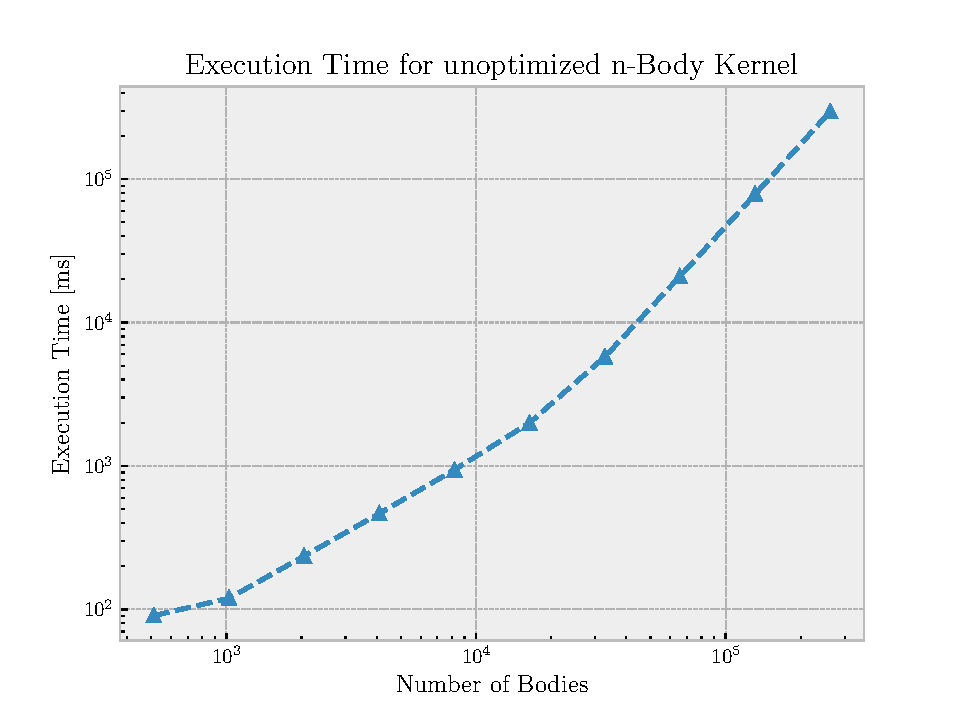
\includegraphics[width=0.9\linewidth]{./plot/time_vs_elems_unopt.pdf}
	\caption{Execution times for unoptimized n-body kernel}%
	\label{fig:time_vs_elems_unopt}
\end{figure}
For the first exercise we implemented a naive kernel for a n-Body simulation. The measurements are shown in Figure \ref{fig:time_vs_elems_unopt}. We can definitely see the $\mathcal O(N^2)$ scaling behavior of the algorithm.

\subsection{Optimized GPU implementation}
\begin{figure}[H]
	\centering
	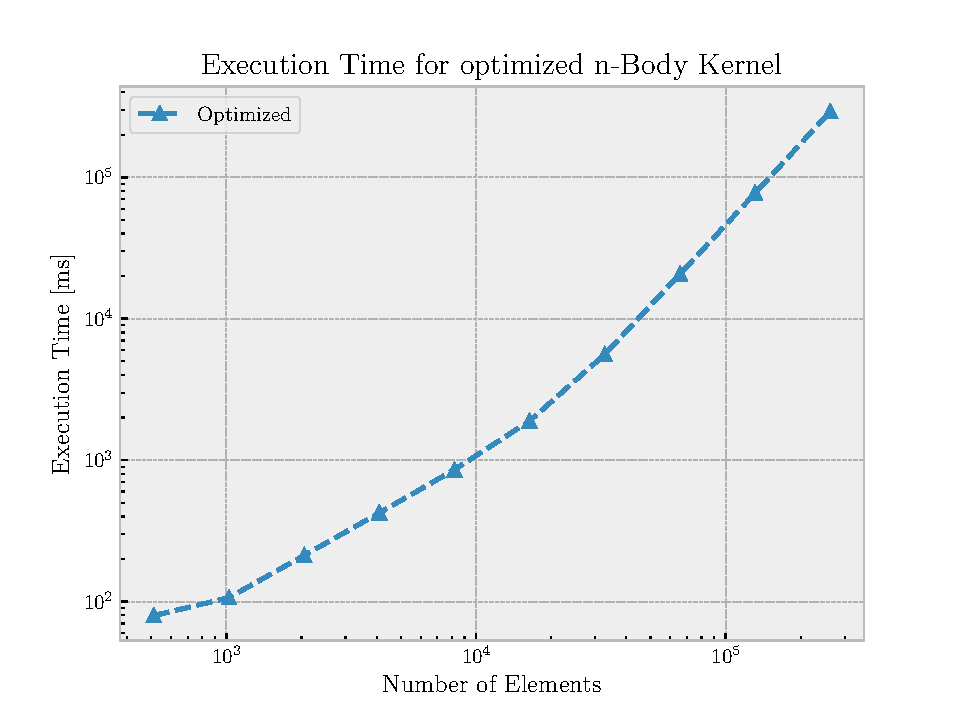
\includegraphics[width=0.9\linewidth]{./plot/time_vs_elems_opt.pdf}
	\caption{Execution times for unoptimized n-body kernel}%
	\label{fig:time_vs_elems_opt}
\end{figure}
For the optimized implementation we decided to use structure of arrays for the better access pattern and tried to use tiling to optimize for shared memory use. We also were trying to use loop unrolling, but this always decreased our performance. The results are shown in Figure \ref{fig:time_vs_elems_opt} and \ref{fig:time_vs_elems_both}. We can only observe an increasing performance for smaller number of bodies. Maybe the additional writing in shared memory and synchronization steps are limiting the performance.

\begin{figure}[H]
	\centering
	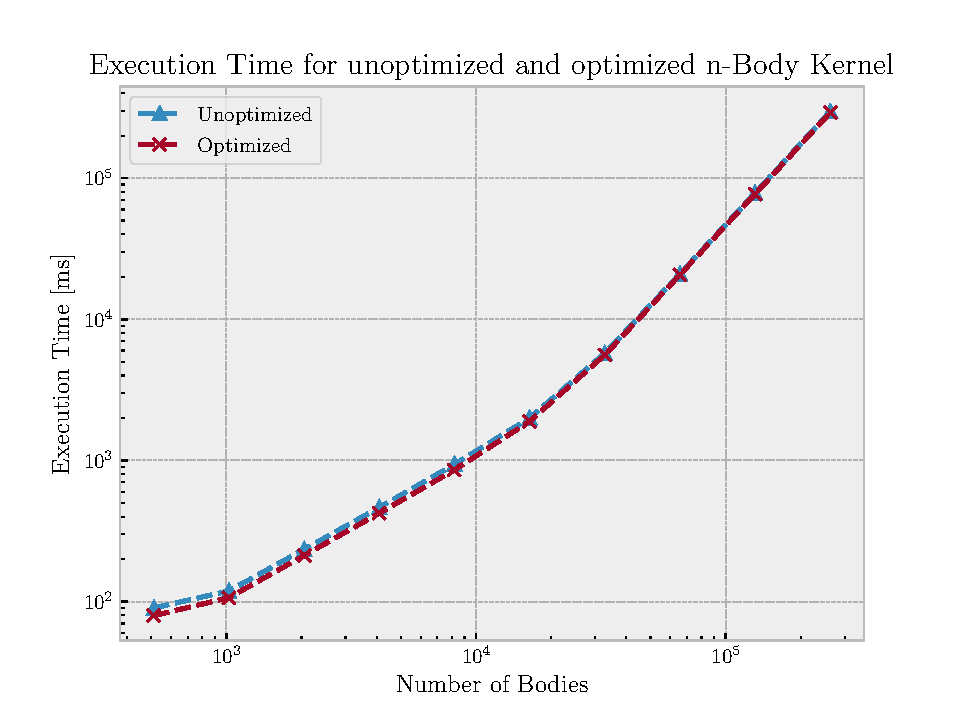
\includegraphics[width=0.9\linewidth]{./plot/time_vs_elems_both.pdf}
	\caption{Comparison of execution times for optimized and unoptimized versions}%
	\label{fig:time_vs_elems_both}
\end{figure}

\subsection{n-Body GPU computations and streaming}

\begin{figure}[H]
	\centering
	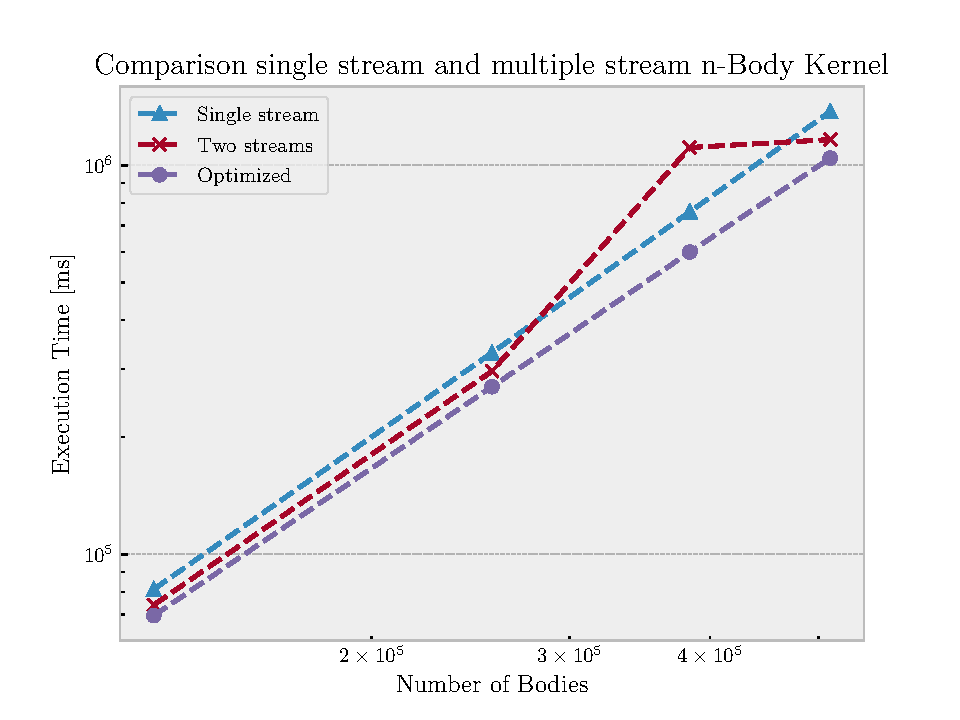
\includegraphics[width=0.9\linewidth]{./plot/streams.pdf}
	\caption{Execution times for n-body kernel using one and two streams}%
	\label{fig:streams}
\end{figure}

For the last part we artificially limited the memory of the GPU to 4MB or to be more precise to hold a total amount of 128k bodies. To solve larger problems the host memory is acting as a swap space. To overlap the kernel execution with the memcpy operation we were using two streams, as more streams would split up the memory in even smaller parts. We were varying the segment size of our device memory between the persistent data and the swapped data but did not observe any big difference. The results are shown in Figure \ref{fig:streams}. As one can see the optimized version from exercise 7.2 is faster since there is no memory limit. However, even the single streamed version is faster than our two stream implementation, which is bit strange, but for a large amount of bodies the two stream version gets faster.

\subsection{Willingness to present}
Hereby, we declare our will to present the results shown in the former sections.


\end{document}
